\chapter[Thực nghiệm, kết quả và phân tích]{Thực nghiệm,\\kết quả và phân tích}
\label{chap:results}

Chương này trình bày toàn diện các kết quả thực nghiệm nhằm kiểm chứng từng giả thuyết thiết kế của Chương~\ref{chap:method}, bám sát theo mạch năm câu hỏi nghiên cứu (RQ1--RQ5) đã đề ra. Nhằm bảo đảm tính khách quan và minh bạch, các thực nghiệm được triển khai theo lộ trình từ đơn giản đến hoàn chỉnh: (1) đánh giá vai trò của chuỗi dữ liệu dọc và giá trị bổ sung từ đa phương thức (RQ1--RQ2); (2) kiểm nghiệm ưu thế của tương tác song tuyến theo cặp so với phương thức ghép nối cơ sở (RQ3); (3) lượng hóa mức độ cắt giảm tham số của phân rã CP và tính ưu việt của cấu trúc tinh giản RC-Free khi đối chiếu với toàn bộ bảy tổ hợp tương tác cùng quy trình tham chiếu (RQ4--RQ5); và (4) kiểm chứng năng lực phân tầng sống còn thực tế của mô hình RC-Free thông qua các thước đo IPCW-AUC theo thời hạn và đường cong Kaplan--Meier.

\section{Thiết lập huấn luyện và diễn biến hội tụ}
\label{sec:experimental-protocol}
Mọi thực nghiệm trong khóa luận đều sử dụng nhất quán cách phân chia cố định theo mã định danh người tham gia đã trình bày ở Mục~\ref{sec:data-split} (gồm 251 người thuộc tập huấn luyện, 54 người thuộc tập xác thực và 54 người thuộc tập kiểm tra hậu nghiệm; tương ứng với 74, 16 và 16 ca biến cố), trong đó toàn bộ tham số tiền xử lý chỉ được khớp duy nhất trên tập huấn luyện. Tập xác thực có 480 cặp so sánh hợp lệ và tập kiểm tra hậu nghiệm có 528 cặp. Loạt thí nghiệm thăm dò đầu vào ban đầu (RQ1--RQ2) được thực hiện trên một lần khởi tạo; toàn bộ các so sánh kiến trúc cốt lõi và đánh giá sống còn chuyên sâu sau đó đều được lặp lại qua ba mã khởi tạo ngẫu nhiên độc lập (seed 20260727, 20260728 và 20260729), với kết quả được báo cáo dưới dạng giá trị trung bình $\pm$ độ lệch chuẩn mẫu (SD).

Do dữ liệu ảnh thể tích MRI 3D chiếm dụng dung lượng bộ nhớ GPU rất lớn trong khi hàm mất mát sống còn Cox lại nhạy cảm với kích thước lô nhỏ, quy trình huấn luyện được tôi thiết lập hết sức cẩn trọng như sau:
\begin{enumerate}
\item \emph{Thuật toán tối ưu hóa}: Sử dụng thuật toán AdamW \cite{loshchilov2019adamw} với tốc độ học ban đầu $10^{-4}$, hệ số suy giảm trọng số (weight decay) $10^{-4}$, bộ tham số mô-men $(\beta_1,\beta_2)=(0.9,0.999)$ và áp dụng kỹ thuật cắt chuẩn gradient tại ngưỡng $1.0$ \cite{pascanu2013difficulty} để bảo đảm tính ổn định khi tối ưu.
\item \emph{Cỡ lô, tích lũy gradient và độ chính xác hỗn hợp}: Cỡ lô cơ sở được đặt bằng 6 người kết hợp kỹ thuật tích lũy gradient qua 2 lô trước mỗi bước cập nhật trọng số (tập nguy cơ Cox được tính riêng trên từng lô cụ thể). Quá trình huấn luyện ứng dụng kỹ thuật độ chính xác hỗn hợp FP16 \cite{micikevicius2018mixed} nhằm tiết kiệm bộ nhớ, riêng các phép tính log-sum-exp trong hàm mất mát Cox được ép kiểu về FP32 để bảo đảm độ chính xác số học.
\item \emph{Bộ lấy mẫu lô hợp lệ cho hàm mất mát Cox}: Bộ lấy mẫu được thiết kế chuyên biệt sao cho mỗi người bệnh xuất hiện đúng một lần trong mỗi vòng huấn luyện (tổng cộng 42 lô/vòng) và mỗi lô dữ liệu luôn bảo đảm chứa ít nhất một cặp cá thể có thể so sánh hợp lệ. Nhờ đó, xuyên suốt cả ba lần khởi tạo ngẫu nhiên, toàn bộ 4032 lượt cập nhật lô huấn luyện đều diễn ra hợp lệ tuyệt đối.
\item \emph{Điều chỉnh tốc độ học và tiêu chí chọn mô hình}: Mô hình được huấn luyện tối đa 100 vòng với bộ điều chỉnh \texttt{ReduceLROnPlateau} \cite{pytorchReduceLROnPlateau} theo dõi hàm mất mát Cox trên tập xác thực (giảm một nửa tốc độ học nếu sau 5 vòng không ghi nhận cải thiện, với mức sàn tối thiểu là $10^{-6}$). Sau 10 vòng khởi động ban đầu, cơ chế dừng sớm được kích hoạt dựa trên chỉ số C-index xác thực (ngưỡng cải thiện tối thiểu là 0.002, số vòng chờ tối đa là 20); mô hình được lưu lại là checkpoint đạt C-index xác thực cao nhất.
\end{enumerate}

\begin{figure}[H]
\centering
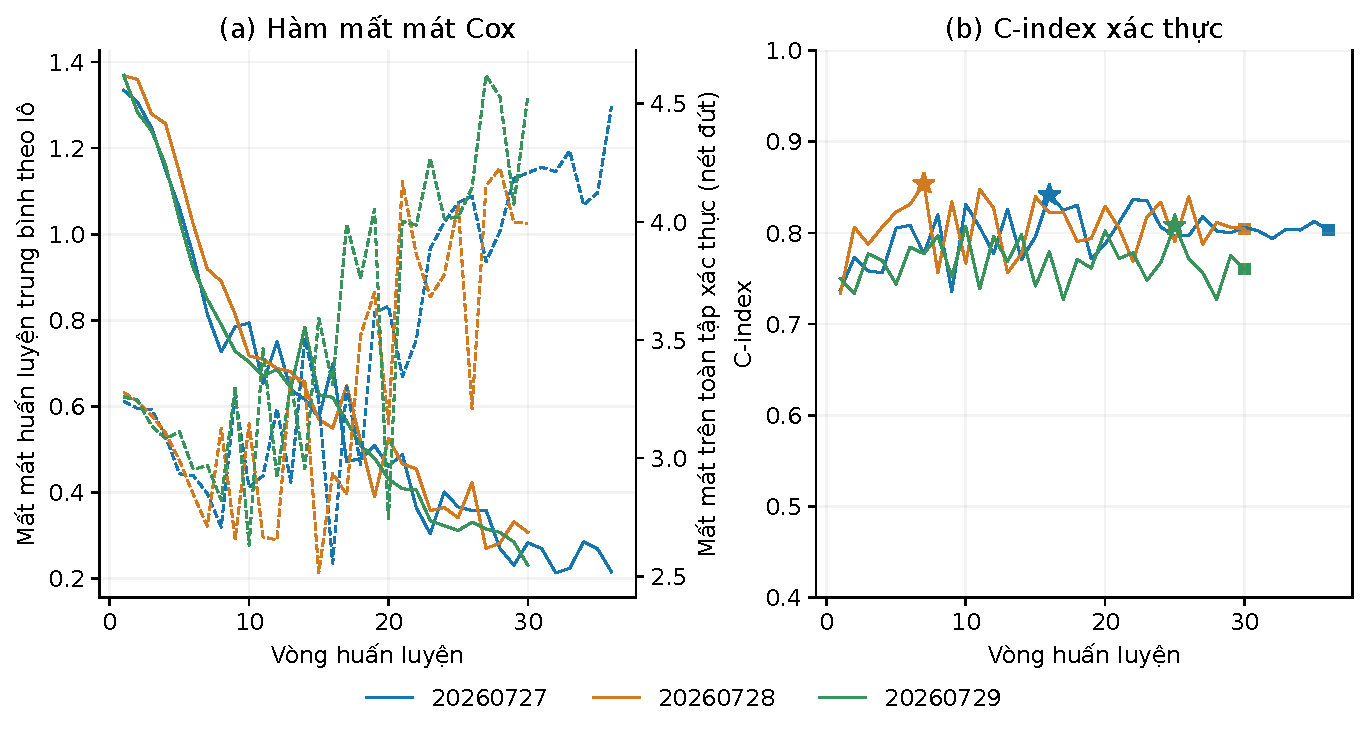
\includegraphics[width=\textwidth]{image/empirical-training.pdf}
\caption{Diễn biến huấn luyện của mô hình RC-Free qua ba lần khởi tạo}
\label{fig:empirical-training}
\captionsetup{justification=raggedright}
\caption*{Ô (a): hàm mất mát huấn luyện trung bình theo lô (đường liền, trục trái) và hàm mất mát xác thực trên toàn tập (đường đứt, trục phải). Ô (b): C-index xác thực theo từng vòng; dấu sao là mô hình được chọn, hình vuông là vòng dừng sớm.}
\end{figure}

Diễn biến huấn luyện ở Hình~\ref{fig:empirical-training} cho thấy trên cả ba lượt chạy, hàm mất mát huấn luyện hội tụ đều đặn (giảm từ 1.33--1.37 xuống 0.22--0.31), trong khi hàm mất mát trên tập xác thực có xu hướng tăng dần sau một số vòng đầu (từ 3.24--3.28 lên 3.99--4.53) — một dấu hiệu điển hình của hiện tượng quá khớp khi tối ưu mạng học sâu trên cỡ mẫu y tế hạn chế. Cần nhấn mạnh rằng, chúng ta không nên so sánh trực tiếp trị số tuyệt đối giữa hai đường mất mát này, bởi giá trị của hàm mất mát đối log-hợp lý Cox phụ thuộc chặt chẽ vào kích thước của tập nguy cơ \cite{kvamme2019time} (vốn chỉ có tối đa 6 người trong mỗi lô huấn luyện nhỏ, so với toàn bộ 54 người trên tập xác thực). Xuất phát từ mục tiêu tối hậu của bài toán là xếp hạng nguy cơ, tôi tiến hành chọn mô hình tối ưu dựa trên điểm cực đại của chỉ số C-index xác thực (ô b): ba lượt chạy tương ứng đã xác định các điểm dừng checkpoint tại các vòng 16, 7 và 25 (đạt C-index xác thực lần lượt là 0.8417, 0.8542 và 0.8083) và kích hoạt cơ chế dừng sớm tại các vòng 36, 30 và 30.

\section{Vai trò của dữ liệu dọc và đa phương thức (RQ1--RQ2)}
Trước hết, để thiết lập nền tảng thực nghiệm vững chắc, tôi tiến hành loạt thí nghiệm thăm dò nhằm trả lời hai câu hỏi nghiên cứu đầu tiên: liệu thông tin dọc từ chuỗi chụp lặp lại và sự bổ sung của radiomics cùng điểm lâm sàng có thực sự cải thiện năng lực xếp hạng nguy cơ hay không. Bảng~\ref{tab:exploratory} tổng hợp kết quả đo lường C-index xác thực trên các cấu hình mô hình tăng dần (sử dụng seed 20260727).

\begin{table}[H]
\centering\small
\caption[So sánh cấu hình đầu vào cho RQ1--RQ2]{C-index xác thực của các cấu hình đầu vào tăng dần (seed 20260727).}
\label{tab:exploratory}
\begin{tabularx}{\linewidth}{@{}Y r@{}}
\toprule
\textbf{Cấu hình mô hình} & \textbf{C-index $\uparrow$} \\
\midrule
MRI cuối (đơn thời điểm) & 0.7333 \\
MRI dọc và T-LSTM & 0.7333 \\
MRI dọc, T-LSTM và attention & 0.7833 \\
Ghép nối ba nguồn dữ liệu (MRI + Radiomics + Lâm sàng) & \textbf{0.8125} \\
\bottomrule
\end{tabularx}
\end{table}

Các số liệu thực nghiệm ghi nhận hai bước tiến hiệu năng rõ rệt. Thứ nhất, việc chỉ sử dụng trạng thái ẩn cuối cùng của mạng T-LSTM trên ba ảnh MRI chưa thể vượt qua mô hình chỉ dùng ảnh chụp cắt ngang tại thời điểm cuối (cùng đạt mức 0.7333); tuy nhiên, ngay khi tích hợp thêm cơ chế chú ý (attention) để tổng hợp có trọng số toàn bộ ba lần khám, C-index đã tăng vọt từ 0.7333 lên 0.7833 (+0.0500 điểm). Phát hiện này khẳng định giá trị tiên lượng của dữ liệu dọc chỉ thực sự được khai phóng khi mô hình có khả năng tự động cân đối mức độ đóng góp thông tin giữa các thời điểm khám thay vì phụ thuộc thụ động vào bước cuối cùng. Thứ hai, khi bổ sung đồng thời đặc trưng radiomics và các thang điểm lâm sàng thông qua phép ghép nối đặc trưng đơn giản, chỉ số C-index tiếp tục được nâng lên mức \textbf{0.8125} (tăng thêm +0.0292 điểm so với cấu hình chỉ dùng chuỗi MRI tốt nhất). Dựa trên cơ sở thực nghiệm vững chắc này, toàn bộ các thí nghiệm chuyên sâu tiếp theo được tôi thiết lập mặc định với sự hiện diện đồng thời của cả ba nguồn dữ liệu kết hợp mạng T-LSTM và cơ chế attention.

\section{Đối chiếu ghép nối và tương tác tích ngoài (RQ3)}
\label{sec:matched-fusion}
Sau khi đã khẳng định vai trò không thể tách rời của cả ba nguồn dữ liệu dọc, tôi tiếp tục kiểm chứng câu hỏi nghiên cứu thứ ba (RQ3): liệu việc mô hình hóa tường minh tương tác song tuyến bằng phép tích ngoài có mang lại hiệu quả vượt trội so với phương thức ghép nối đặc trưng truyền thống hay không. Để cô lập tuyệt đối và đánh giá chính xác tác động thuần túy của cơ chế hợp nhất, tôi cố định toàn bộ các thành phần kiến trúc còn lại (gồm bộ mã hóa ResNet-18 3D, mạng T-LSTM ẩn 128 chiều, cơ chế attention, hàm mục tiêu Cox Breslow và toàn bộ siêu tham số huấn luyện), đồng thời bảo đảm khởi tạo \emph{chính xác cùng một bộ trọng số ban đầu} cho các phần kiến trúc dùng chung ở mỗi lần chạy (Bảng~\ref{tab:matched-fusion}).

\begin{table}[H]
\centering\small
\caption[So sánh ghép nối và tích ngoài]{C-index xác thực của ghép nối và tích ngoài khi giữ cùng trọng số khởi tạo cho các phần chung (trung bình $\pm$ SD qua ba lần chạy).}
\label{tab:matched-fusion}
\begin{tabularx}{\linewidth}{@{}Y r@{}}
\toprule
\textbf{Cấu trúc hợp nhất} & \textbf{C-index $\uparrow$} \\
\midrule
Concatenation (ghép nối) & $0.8149\pm0.0214$ \\
Full Outer-Product (tích ngoài đầy đủ) & $\mathbf{0.8285\pm0.0272}$ \\
\bottomrule
\end{tabularx}
\end{table}

Dưới các điều kiện kiểm soát nghiêm ngặt và đồng nhất về trọng số khởi tạo ban đầu, biến thể Full Outer-Product đạt C-index xác thực trung bình là \textbf{0.8285}, vượt trội hơn mức 0.8149 của phương thức ghép nối cơ bản (mức chênh lệch trung bình đạt \textbf{0.0135} tính trên giá trị chưa làm tròn). Mức cải thiện ổn định này minh chứng rằng việc mô hình hóa tường minh các tích chéo bậc hai giúp mạng nơ-ron khai thác sâu sắc và hiệu quả hơn các mối liên kết tiềm ẩn giữa ba nguồn dữ liệu. Đây chính là tiền đề quan trọng để tôi lựa chọn Full Outer-Product làm mốc chuẩn tham chiếu cho hai bước tinh giản kế tiếp: nén tham số bằng phân rã CP và loại bỏ các tương tác dư thừa.

\section{Phân rã CP, RC-Free và đối chiếu (RQ4--RQ5)}
\label{sec:cp-results}
\label{sec:ablation-results}
\label{sec:rcfree-multiseed}
\label{sec:standardized-benchmark}
\label{sec:paper-adaptation-results}

Xuất phát từ cấu trúc Full Outer-Product, tôi tiến hành hai bước tinh giản kiến trúc có kiểm soát trên cùng bộ ba seed ngẫu nhiên (20260727--20260729), sau đó đặt mô hình đề xuất cạnh quy trình tham chiếu chuẩn mực CNN--PCA--T-LSTM nhằm giải quyết trọn vẹn RQ4 và RQ5.

\subsection{Mức giảm tham số nhờ phân rã CP (RQ4)}
\label{sec:computational-efficiency}
Khi chuyển đổi từ Full Outer-Product sang Full CP, toàn bộ các bộ mã hóa phương thức, các nhánh phần dư có cổng điều tiết và khối thời gian phía sau đều được giữ nguyên vẹn; sự thay đổi duy nhất nằm ở việc lớp song tuyến đầu tiên của ba cặp MR, MC và RC được tham số hóa thông qua phân rã CP với hạng lần lượt là 8, 8 và 4 (Bảng~\ref{tab:cpconfig}). Bảng~\ref{tab:interaction-parameters} đối chiếu cụ thể số lượng tham số ở ba phạm vi kiến trúc khác nhau.

\begin{table}[H]
\centering\small
\caption[Tham số tương tác và toàn mạng]{Số tham số của Full Outer-Product và Full CP ở ba phạm vi (gồm độ chệch).}
\label{tab:interaction-parameters}
\begin{tabularx}{\linewidth}{@{}Y r r@{}}
\toprule
\textbf{Phạm vi} & \textbf{Full Outer-Product} & \textbf{Full CP} \\
\midrule
Ba lớp song tuyến đầu & 229696 & \textbf{3712} \\
Ba khối tương tác, gồm MLP & 248608 & \textbf{22624} \\
Toàn mạng & 33760941 & \textbf{33534957} \\
\bottomrule
\end{tabularx}
\end{table}

Số liệu ở Bảng~\ref{tab:interaction-parameters} phản ánh sinh động hiệu quả nén tham số vượt trội của kỹ thuật phân rã CP: tại đúng ba lớp song tuyến đầu tiên, số lượng trọng số cần tối ưu giảm ngoạn mục từ 229696 xuống chỉ còn 3712 tham số, tương ứng với tỷ lệ cắt giảm lên tới \textbf{98.38\%}; khi tính chung cho toàn bộ khối tương tác (bao gồm cả các tầng MLP phía sau), mức cắt giảm vẫn đạt con số ấn tượng \textbf{90.90\%}. Ngược lại, xét trên quy mô toàn mạng, tỷ lệ suy giảm chỉ đạt khoảng 0.67\% do kiến trúc xương sống ResNet-18 3D của nhánh ảnh MRI chiếm tỷ trọng áp đảo và không thay đổi. Đổi lại sự tinh giản cấu trúc triệt để tại tầng tương tác, chỉ số C-index xác thực trung bình của Full CP (0.8278) chỉ thấp hơn Full Outer-Product (0.8344) một khoảng rất nhỏ là 0.0066 trên loạt đối sánh chính (Bảng~\ref{tab:standard-bench}). Thay vì chấp nhận dừng lại ở Full CP, bước nghiên cứu tiếp theo sẽ kiểm chứng xem liệu việc loại bỏ các tương tác dư thừa có thể giúp mô hình vừa tiết kiệm thêm tham số, vừa phục hồi hoàn toàn năng lực xếp hạng hay không.

\subsection{So sánh bảy cấu trúc tương tác cặp và lựa chọn RC-Free (RQ5)}
\label{sec:new-topology}
Để kiểm nghiệm giả thuyết rằng không nhất thiết phải duy trì đầy đủ cả ba cặp tương tác, tôi tiến hành khảo sát toàn diện mọi tổ hợp cấu trúc CP có ít nhất một cặp tương tác đang hoạt động (gồm ba cấu hình 1 cặp, ba cấu hình 2 cặp và cấu hình Full CP 3 cặp). Điểm cốt lõi cần nhấn mạnh là: \emph{tất cả các cấu trúc này đều bảo tồn trọn vẹn cả ba nguồn dữ liệu đầu vào cùng các đường truyền biểu diễn gốc}; sai khác duy nhất chỉ nằm ở việc cặp tương tác song tuyến nào được kích hoạt. Bảng~\ref{tab:new-topology} tổng hợp chi tiết kết quả thực nghiệm qua ba lần khởi tạo ngẫu nhiên.

\begin{table}[H]
\centering\small
\caption[So sánh bảy cấu trúc có tương tác cặp]{Số tham số toàn mạng và C-index xác thực của bảy cấu trúc CP có tương tác cặp (trung bình $\pm$ SD qua ba lần khởi tạo).}
\label{tab:new-topology}
\begin{tabularx}{\linewidth}{@{}Y c r r@{}}
\toprule
\textbf{Cấu trúc} & \textbf{Cặp / nhánh} & \textbf{Số tham số} & \textbf{C-index $\uparrow$} \\
\midrule
MR-only & 1 / 2 & 33484165 & $0.8299\pm0.0267$ \\
MC-only & 1 / 2 & 33484037 & $0.8236\pm0.0237$ \\
RC-only & 1 / 2 & 33464165 & $0.8319\pm0.0214$ \\
RC-Free (MR+MC) & 2 / 4 & 33519497 & $\mathbf{0.8347\pm0.0237}$ \\
MR-Free (MC+RC) & 2 / 4 & 33499625 & $0.8243\pm0.0249$ \\
MC-Free (MR+RC) & 2 / 4 & 33499753 & $0.8222\pm0.0156$ \\
Full CP & 3 / 6 & 33534957 & $0.8278\pm0.0250$ \\
\bottomrule
\end{tabularx}
\end{table}

Trong toàn bộ bảy cấu hình khảo sát, kiến trúc \textbf{RC-Free (MR+MC)} đã xác lập chỉ số C-index xác thực trung bình cao nhất (\textbf{0.8347}), theo sau là cấu hình một cặp RC-only (0.8319). Đáng chú ý, khi đặt cạnh cấu trúc Full CP, việc chủ động loại bỏ cặp tương tác trực tiếp RC không chỉ giúp tinh giản số nhánh phần dư từ sáu xuống bốn nhánh và \textbf{tiết kiệm thêm 15460 tham số}, mà còn trực tiếp nâng C-index trung bình từ 0.8278 lên 0.8347. Cân nhắc đồng thời giữa tính chặt chẽ về mặt cơ chế y sinh (đặt ảnh MRI làm trung tâm kết nối), năng lực phân tầng sống còn vượt trội và độ tinh gọn tham số, kiến trúc RC-Free chính là giải pháp tối ưu nhất để đưa vào phân tích sống còn chuyên sâu.

\subsection{Đối chiếu tổng thể với quy trình tham chiếu}
Bảng~\ref{tab:standard-bench} tiến hành đối sánh tổng thể mô hình RC-Free đề xuất với Full Outer-Product, Full CP và bản tái lập có điều chỉnh quy trình CNN--PCA--T-LSTM của Aghajanian và cộng sự trên cùng một tập dữ liệu xác thực chuẩn mực.

\begin{table}[H]
\centering\small
\caption[So sánh C-index và độ phức tạp mô hình]{C-index xác thực dưới dạng trung bình $\pm$ SD qua ba lần khởi tạo.}
\label{tab:standard-bench}
\begin{tabularx}{\linewidth}{@{}Y r r c@{}}
\toprule
\textbf{Mô hình} & \textbf{C-index $\uparrow$} & \textbf{Số tham số} & \textbf{Cặp/nhánh} \\
\midrule
CNN--PCA--T-LSTM & $0.7417\pm0.0693$ & $33213122$ & 0 / 0 \\
Full Outer-Product & $0.8344\pm0.0148$ & $33760941$ & 3 / 6 \\
Full CP Pairwise & $0.8278\pm0.0250$ & $33534957$ & 3 / 6 \\
RC-Free Pairwise & $\mathbf{0.8347\pm0.0237}$ & $33519497$ & 2 / 4 \\
\bottomrule
\end{tabularx}
\caption*{\textit{Ghi chú.} Các số liệu trong bảng do khóa luận tính trên cùng tập xác thực. Mô hình đối chứng CNN--PCA--T-LSTM được xây dựng theo quy trình của Aghajanian và cộng sự~\cite{aghajanian2025longitudinal}, với các điều chỉnh ở Bảng~\ref{tab:reference-methods}.}
\end{table}


So với cấu trúc Full Outer-Product, mô hình RC-Free \textbf{cắt giảm được 241444 tham số} (nhờ tinh giản từ 3 cặp / 6 nhánh xuống còn 2 cặp / 4 nhánh) trong khi vẫn xác lập C-index trung bình cao hơn (\textbf{0.8347} so với 0.8344). Đặc biệt, khi đối chiếu với quy trình tham chiếu CNN--PCA--T-LSTM ($0.7417\pm0.0693$), cả ba biến thể hợp nhất đa phương thức đầu-cuối đều đạt C-index vượt trội hơn hẳn từ 0.086 đến 0.093 điểm, đồng thời độ lệch chuẩn giữa ba lần khởi tạo giảm gần ba lần (0.0148--0.0250 so với 0.0693). Kết quả thực nghiệm vững chắc này chứng minh rằng quy trình huấn luyện đầu-cuối kết hợp bộ mã hóa tiền huấn luyện và cơ chế tương tác đa nguồn đem lại sự bứt phá vượt bậc cả về độ chính xác xếp hạng lẫn tính ổn định số học so với mô hình hai bước truyền thống dựa trên đặc trưng nén PCA.

\section{Phân tích sống còn của RC-Free}
\label{sec:posthoc-test}
\label{sec:survival-results}
Với kiến trúc RC-Free tối ưu đã được lựa chọn, phần này kiểm chứng chuyên sâu chất lượng của điểm log-nguy cơ $\eta_i$ trên cả tập xác thực (đánh giá chính) và tập kiểm tra hậu nghiệm độc lập theo hai khía cạnh bổ trợ: khả năng phân biệt tại từng thời hạn lâm sàng (IPCW-AUC) và năng lực phân tầng nhóm nguy cơ theo thời gian (Kaplan--Meier).

\subsection{C-index và AUC theo thời gian tại 2, 3 và 5 năm}
Bảng~\ref{tab:survival-metrics} tổng hợp chi tiết chỉ số C-index cùng các giá trị AUC tại ba mốc thời gian then chốt, đi kèm Bảng~\ref{tab:horizon-support} thống kê cụ thể số ca biến cố, số đối chứng và số ca kiểm duyệt tại từng thời điểm nhằm làm rõ bối cảnh mẫu của các ước lượng.

\begin{table}[H]
\centering\small
\caption[C-index và AUC của RC-Free]{C-index và AUC của RC-Free, trình bày dưới dạng trung bình $\pm$ SD qua ba lần khởi tạo. Mỗi tập gồm 54 người với 16 biến cố.}
\label{tab:survival-metrics}
\begin{tabularx}{\linewidth}{@{}Y r r@{}}
\toprule
\textbf{Chỉ số} & \textbf{Xác thực (chính)} & \textbf{Kiểm tra (hậu nghiệm)} \\
\midrule
C-index & $\mathbf{0.8347\pm0.0237}$ & $\mathbf{0.8466\pm0.0267}$ \\
AUC 2 năm & $\mathbf{0.9805\pm0.0149}$ & $0.8858\pm0.0245$ \\
AUC 3 năm & $\mathbf{0.9788\pm0.0162}$ & $0.8770\pm0.0318$ \\
AUC 5 năm & $0.7889\pm0.0632$ & $0.8483\pm0.0508$ \\
\bottomrule
\end{tabularx}
\end{table}

\begin{table}[H]
\centering\small
\caption[Số người theo trạng thái và xác suất chưa kiểm duyệt tại từng mốc]{Tại mỗi mốc, ba số lần lượt là số người có biến cố tính đến mốc, số người được theo dõi quá mốc và số người bị kiểm duyệt trước hoặc tại mốc. Xác suất chưa bị kiểm duyệt $\widehat G(h)$ được ước lượng từ tập huấn luyện.}
\label{tab:horizon-support}
\begin{tabularx}{\linewidth}{@{}c Y Y r@{}}
\toprule
\textbf{Năm} & \textbf{Xác thực} & \textbf{Kiểm tra (hậu nghiệm)} & \textbf{$\widehat G(h)$} \\
\midrule
2 & 7 / 37 / 10 & 8 / 37 / 9 & $0.831$ \\
3 & 7 / 34 / 13 & 11 / 29 / 14 & $0.697$ \\
5 & 12 / 19 / 23 & 14 / 16 / 24 & $0.475$ \\
\bottomrule
\end{tabularx}
\end{table}


Trên tập xác thực, RC-Free đạt năng lực phân biệt xuất sắc ở các mốc thời gian gần, ghi nhận AUC đạt \textbf{0.9805} tại mốc 2 năm và \textbf{0.9788} tại mốc 3 năm, trước khi đạt 0.7889 tại mốc 5 năm. Khi đối chiếu với dữ liệu thống kê mẫu ở Bảng~\ref{tab:horizon-support}, sự biến thiên này phản ánh trung thực đặc điểm cấu trúc mẫu tại từng thời điểm. Tại các mốc 2 và 3 năm, tập xác thực chỉ ghi nhận \textbf{7 biến cố tích lũy}, do đó các ước lượng thống kê trên cỡ mẫu nhỏ tự nhiên có độ biến động nhất định. Đến mốc 5 năm, mặc dù số ca biến cố tích lũy đã tăng lên 12 trường hợp, số người còn tiếp tục được theo dõi sau 5 năm lại giảm mạnh từ 37 xuống còn 19 người do 23 đối tượng đã bị kiểm duyệt phải trước đó. Biểu đồ ở Hình~\ref{fig:empirical-roc} minh họa trực quan xu hướng này: tại mốc 5 năm trên tập xác thực, các đường cong ROC giữa ba lần khởi tạo có độ phân tán rộng hơn (độ lệch chuẩn SD tăng lên 0.0632) so với sự hội tụ cao ở hai mốc đầu. Đáng mừng là trên tập kiểm tra hậu nghiệm độc lập, mô hình thể hiện tính ổn định cao xuyên suốt cả ba mốc thời gian (với các giá trị AUC lần lượt là 0.8858, 0.8770 và 0.8483) cùng chỉ số C-index tổng thể đạt $0.8466\pm0.0267$.

\begin{figure}[H]
\centering
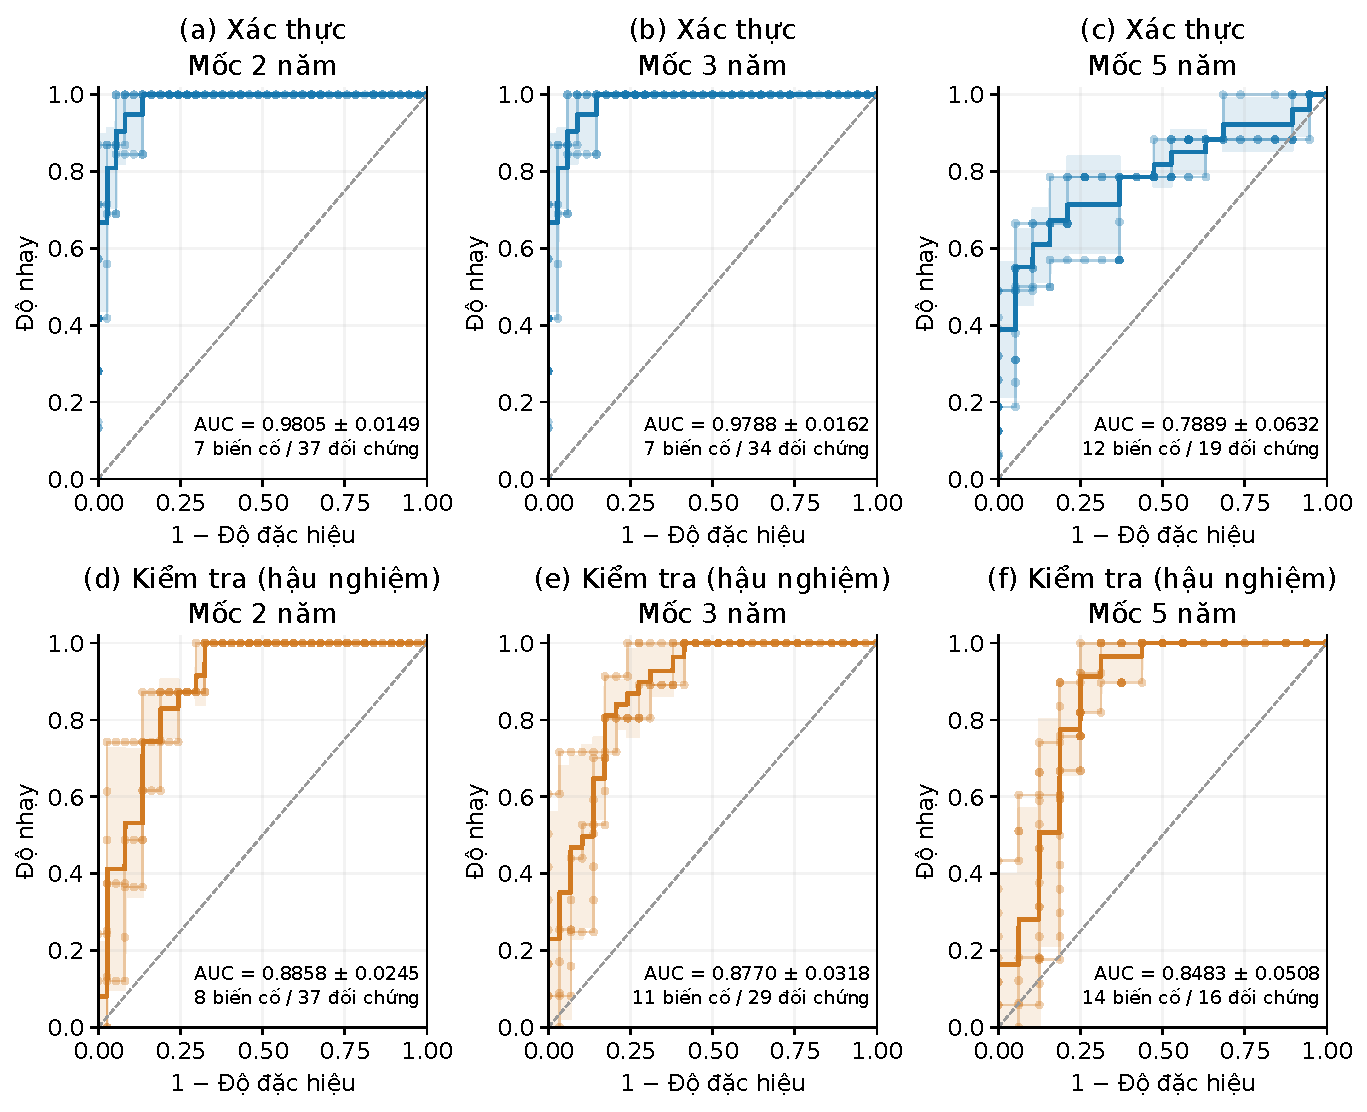
\includegraphics[width=\textwidth]{image/empirical-ipcw-roc.pdf}
\caption{Đường cong ROC có trọng số IPCW của RC-Free tại 2, 3 và 5 năm}
\label{fig:empirical-roc}
\captionsetup{justification=raggedright}
\caption*{Hàng trên: tập xác thực; hàng dưới: tập kiểm tra hậu nghiệm. Đường mảnh và chấm tròn là từng lần chạy; đường đậm là trung bình; vùng tô là $\pm1$ SD. Đường chéo biểu thị mức đoán ngẫu nhiên.}
\end{figure}

\clearpage
\subsection{Phân tầng Kaplan--Meier theo nhóm nguy cơ đồng thuận}
Hình~\ref{fig:survival-km} và Bảng~\ref{tab:km-statistics} đánh giá năng lực tách biệt giữa hai nhóm người bệnh có nguy cơ cao và thấp (được phân định dựa trên ngưỡng trung vị của tập huấn luyện và cơ chế biểu quyết đồng thuận đa số qua ba lần chạy).

\begin{figure}[H]
\centering
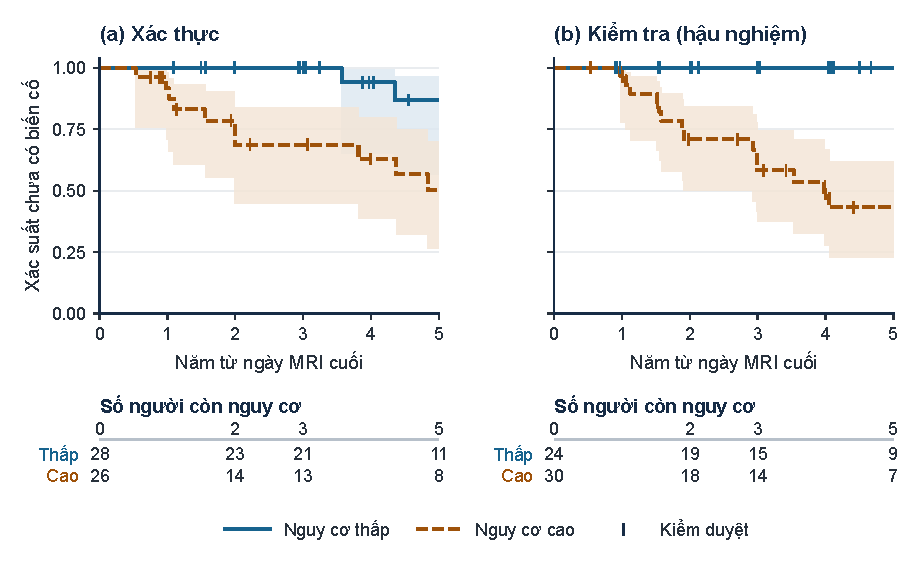
\includegraphics[width=\textwidth]{image/survival-km.pdf}
\caption{Đường cong Kaplan--Meier theo nhóm nguy cơ đồng thuận của RC-Free}
\label{fig:survival-km}
\captionsetup{justification=raggedright}
\caption*{Ô (a): tập xác thực; ô (b): tập kiểm tra hậu nghiệm. Vùng tô là khoảng tin cậy 95\%; dấu gạch dọc đánh dấu thời điểm kiểm duyệt. Bảng dưới trục hoành ghi số người còn nguy cơ tại các mốc thời gian.}
\end{figure}

\begin{table}[H]
\centering\small
\caption[Log-rank và HR theo nhóm nguy cơ]{Kiểm định log-rank, tỷ số nguy cơ (HR) của nhóm nguy cơ cao so với nhóm nguy cơ thấp và kiểm tra giả định nguy cơ tỷ lệ (PH).}
\label{tab:km-statistics}
\begin{tabularx}{\linewidth}{@{}Y r r r r@{}}
\toprule
\textbf{Tập} & \textbf{$p$ log-rank} & \textbf{HR} & \textbf{CI 95\%} & \textbf{$p$ (PH)} \\
\midrule
Xác thực & $\mathbf{0.0134}$ & $\mathbf{3.79}$ & $1.22$--$11.78$ & $0.1031$ \\
Kiểm tra (hậu nghiệm) & $\mathbf{<0.001}$ & $\mathbf{16.17}$ & $2.12$--$123.17$ & $0.1592$ \\
\bottomrule
\end{tabularx}
\end{table}


Hai đường cong tách biệt rõ nét trên cả hai tập dữ liệu, khẳng định năng lực phân tầng nguy cơ vượt trội của mô hình. Trên tập xác thực, nhóm nguy cơ thấp (28 người) chỉ ghi nhận 4 biến cố, trong khi nhóm nguy cơ cao (26 người) ghi nhận 12 biến cố — gấp ba lần nhóm thấp; kiểm định log-rank xác nhận sự khác biệt có ý nghĩa thống kê (\textbf{$p=0.0134$}), với tỷ số nguy cơ ước tính \textbf{HR = 3.79} (CI 95\%: 1.22--11.78). Trên tập kiểm tra hậu nghiệm, độ tương phản còn mạnh mẽ hơn: trong 24 người thuộc nhóm nguy cơ thấp gần như không ghi nhận ca suy giảm nào trong hơn 5 năm đầu (chỉ duy nhất 1 biến cố sau năm thứ năm), đối lập với 15 biến cố trong 30 người thuộc nhóm nguy cơ cao, đạt \textbf{log-rank $p<0.001$} và \textbf{HR = 16.17} (CI 95\%: 2.12--123.17). Khoảng tin cậy rộng của HR trên tập kiểm tra bắt nguồn trực tiếp từ việc nhóm nguy cơ thấp chỉ có đúng một biến cố làm mẫu số so sánh; ngay cả cận dưới của khoảng tin cậy 95\% vẫn đạt 2.12, cho thấy nhóm nguy cơ cao vẫn có tốc độ tiến triển cao hơn rõ rệt. Đồng thời, phép kiểm tra phần dư Schoenfeld cho $p=0.1031$ trên tập xác thực và $p=0.1592$ trên tập kiểm tra (đều lớn hơn 0.05), chứng tỏ tỷ lệ nguy cơ giữa hai nhóm duy trì ổn định theo thời gian và khẳng định RC-Free là kiến trúc vừa đạt hiệu quả xếp hạng cao nhất, vừa cho khả năng phân tầng sống còn sắc nét và tin cậy nhất trong toàn bộ các thử nghiệm.

\section{Trả lời các câu hỏi nghiên cứu}
\label{sec:rq-results}
Tổng hợp toàn bộ chuỗi thực nghiệm trên, câu trả lời cho năm câu hỏi nghiên cứu ở Bảng~\ref{tab:rq} như sau:

\begin{description}[leftmargin=1.35cm,labelwidth=1.1cm,itemsep=.3em]
\item[RQ1.] \emph{Dữ liệu dọc}: Chuỗi ba lần chụp MRI cải thiện rõ rệt so với chỉ dùng ảnh cuối khi kết hợp T-LSTM với attention, tăng C-index xác thực từ 0.7333 lên \textbf{0.7833} (Bảng~\ref{tab:exploratory}).
\item[RQ2.] \emph{Đa phương thức}: Bổ sung radiomics và dữ liệu lâm sàng bằng ghép nối tiếp tục nâng C-index xác thực lên \textbf{0.8125} (+0.0292 so với chỉ dùng MRI, Bảng~\ref{tab:exploratory}).
\item[RQ3.] \emph{Tương tác cặp so với ghép nối}: Khi giữ cùng trọng số khởi tạo cho các phần chung, phép tích ngoài đạt C-index xác thực trung bình cao hơn ghép nối \textbf{0.0135} (0.8285 so với 0.8149, Bảng~\ref{tab:matched-fusion}).
\item[RQ4.] \emph{Phân rã CP}: CP giảm \textbf{98.38\%} số tham số ở ba lớp song tuyến đầu (90.90\% ở ba khối tương tác; 0.67\% toàn mạng, Bảng~\ref{tab:interaction-parameters}), đổi lại mức giảm nhỏ 0.0066 C-index giữa Full CP và Full Outer-Product (Bảng~\ref{tab:standard-bench}).
\item[RQ5.] \emph{Tinh gọn thành RC-Free}: Khả thi và hiệu quả. Bỏ cặp RC tiết kiệm thêm \textbf{15460 tham số} so với Full CP, rút từ sáu xuống bốn nhánh và đạt C-index xác thực trung bình cao nhất trong bảy cấu trúc CP (\textbf{0.8347}, Bảng~\ref{tab:new-topology}), đồng thời phân tầng nguy cơ có ý nghĩa thống kê trên đường cong Kaplan--Meier (Bảng~\ref{tab:km-statistics}).
\end{description}
